% !TEX root = Anforderungsliste.tex
\begin{center}
\begin{tabular}{|p{1cm}|p{0.5cm}|p{5cm}|p{5cm}|p{1.5cm}|}\hline
\textbf{Nr.} & \textbf{F M W} & \textbf{Bezeichnung} & \textbf{Werte Daten Erläuterungen Änderungen} & \textbf{Ver- ant- wort- lich}\\\hline
 1 & F & Maximale Fugenbreite zwischen den Spanplatten & <2mm & Alle\\\hline
 2 & F & Maximaler Überstand zwischen den Spanplatten & <2mm & Alle\\ \hline
 3 & F & Minimaler Abstand zu Hindernissen über der Fahrbahn &  $\geq$ 1m & Alle\\\hline
 4 & F & Minimaler Abstand zu Hindernissen um die Fahrbahn &  $\geq$ 50cm & Alle\\\hline
  5 & F & Die Farbe der abzufahrenden Spur ist Grau und wird mit einer weissen gestrichelten Linie von der Gegenfahrbahn getrennt &   & Alle\\ \hline
  6 & F & Die Breite der weissen Mittellinien & 1cm $\pm$ 0.2 cm & Alle\\ \hline
  7 & F & Die Breite der Fahrspur &  20cm $\pm$ 1cm & Alle\\ \hline
  8 & F & Begrenzungen der rechten Fahrspur & \begin{itemize} \item Durch die Trottoirkante gegeben (sofern ein Trottoir vorhanden ist)\item Mit einer weissen Linie markiert \item Nicht gekennzeichnet \end{itemize}  & Alle\\ \hline
  9 & F & Die Breite der weissen Linie an der rechten Fahrspur &  1cm $\pm$ 0.2cm & Alle\\ \hline
  10 & F & Der Abstand der weissen Linie an der rechten Fahrspur zur Mittellinie(jeweils von der Mitte der beiden Linien)&  20cm $\pm$ 1cm & Alle\\ \hline
  11 & F & Minimale Kurvenradius der Strassenmittellinie &  60cm $\pm$ 5cm & Alle\\ \hline
  12 & F & Die Breite des Trottoirs &  9cm $\pm$ 1cm & Alle\\ \hline
  13 & F & Die Höhe der Trottoirkante &  0.5cm $\pm$ 0.1cm & Alle\\ \hline
  14 & F & Das Trottior ist fest und darf belastet werden & & Alle\\ \hline
  15 & F & Der Abstand von den auf dem Trottoir platzierten Objekten (z.B Bauarbeiter, Schranken, etc.) zu den Containern & $\geq$ 10cm & Alle\\ \hline
  16 & F & Die Länge des Start- und Zielparkfeld & 50cm $\pm$ 2cm & Alle\\ \hline
  17 & F & Die Breite des Start- und Zielparkfeld & 20cm $\pm$ 1cm & Alle\\ \hline
  18 & F & Drei Seiten der Start - und Zielfelder werden mit einer weissen Linie markiert. & & Alle\\ \hline
  19 & F & Die Breite der Randlinien der Felder & 1cm $\pm$ 0.2cm & Alle\\ \hline
  20 & F & Die vom Fahrzeug aus gesehene linke Randlinie ist wie die Mittellinie gekennzeichnet & & Alle\\\hline
  21 & F & Es dürfen keine Gegenstände auf der Fahrbahn liegen oder auf die Fahrbahn ragen & & Alle\\\hline
\end{tabular}
\end{center}

\begin{figure}[ht]
	\centering									
	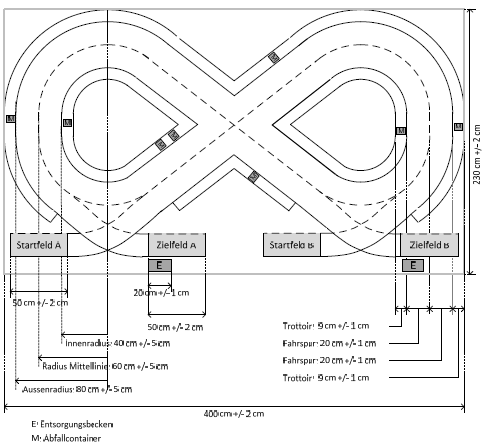
\includegraphics{Images/Fahrbahn.png}
	\caption{Die Fahrbahn mit den Bemasssungen aus der Aufgabenstellung (nicht massstäblich.}
	\label{fig1}
	%Quelle: Aufgabenstellung_PREN1_H15_V2.pdf
\end{figure}